               % final (journal style)
%\documentclass[review,journal]{vgtc}         % review (journal style)
%\documentclass[widereview]{vgtc}             % wide-spaced review
%\documentclass[preprint,journal]{vgtc}       % preprint (journal style)
%\documentclass[electronic,journal]{vgtc}     % electronic version, journal

%% Uncomment one of the lines above depending on where your paper is
%% in the conference process. ``review'' and ``widereview'' are for review
%% submission, ``preprint'' is for pre-publication, and the final version
%% doesn't use a specific qualifier. Further, ``electronic'' includes
%% hyperreferences for more convenient online viewing.

%% Please use one of the ``review'' options in combination with the
%% assigned online id (see below) ONLY if your paper uses a double blind
%% review process. Some conferences, like IEEE Vis and InfoVis, have NOT
%% in the past.

%% Please note that the use of figures other than the optional teaser is not permitted on the first page
%% of the journal version.  Figures should begin on the second page and be
%% in CMYK or Grey scale format, otherwise, colour shifting may occur
%% during the printing process.  Papers submitted with figures other than the optional teaser on the
%% first page will be refused.

%% These three lines bring in essential packages: ``mathptmx'' for Type 1
%% typefaces, ``graphicx'' for inclusion of EPS figures. and ``times''
%% for proper handling of the times font family.



%\chapter{Visual Compression of Workflow Visualizations with Automated Detection of Macro Motifs}
\chapter{Glyph-based Visual Compression of Workflows}
\label{chap:automacron}

\begin{chapquote}{L. Ron Hubbard}{``The evolution of knowledge is toward simplicity, not complexity.''}
\end{chapquote}


%% This is how authors are specified in the journal style

%% indicate IEEE Member or Student Member in form indicated below


%\shortauthortitle{Firstauthor \MakeLowercase{\textit{et al.}}: Paper Title}

%% Abstract section.

 % convincing image showing compression of a repetitive sequence in a workflow using macros.
 


%% Uncomment below to disable the manuscript note
%\renewcommand{\manuscriptnotetxt}{}

%% Copyright space is enabled by default as required by guidelines.
%% It is disabled by the 'review' option or via the following command:
% \nocopyrightspace

%%%%%%%%%%%%%%%%%%%%%%%%%%%%%%%%%%%%%%%%%%%%%%%%%%%%%%%%%%%%%%%%
%%%%%%%%%%%%%%%%%%%%%% START OF THE PAPER %%%%%%%%%%%%%%%%%%%%%%
%%%%%%%%%%%%%%%%%%%%%%%%%%%%%%%%%%%%%%%%%%%%%%%%%%%%%%%%%%%%%%%%%

%% The ``\maketitle'' command must be the first command after the
%% ``\begin{document}'' command. It prepares and prints the title block.

%% the only exception to this rule is the \firstsection command
\section{Introduction}

%% \section{Introduction} %for journal use above \firstsection{..} instead


The term ``macro'' is derived from the Greek word \emph{makro} meaning \emph{big} or \emph{far}.
In Computer Science, the term is defined as ``a single instruction that expands automatically into a set of instruction'' \cite{oxforddict}.
It is commonly used as a noun (\eg, a macro), or an adjective (a macro command). 
In schematic diagrams, such as electronic circuit diagrams, data flow diagrams, and control engineering block diagrams, \emph{macros} are commonly used to provide hierarchical concept abstraction as well as visual compression.
Not only can macros facilitate the ``overview first, details on demand'' from Sheiderman \cite{shneiderman96}, but they can also speed up visual search and reduce cognitive load for experienced users, who are knowledgeable about or have become accustomed to the specification of individual macros.
In effect, their functionality bears some resemblance to \emph{acronyms}.

This work is motivated by the need to reduce the visual complexity of biological experiment workflows in an extension to work conducted in the previous chapter.
Such workflows describe the sequence of processes (arranged with respect to a temporal dimension) enacted on biological materials and signals obtained through experimental observations.
Large repositories of experimental data offer a data corpus that can be tapped into for workflow analysis and, more specifically, detection of commonly-used subgraphs (also referred to as \emph{motifs}).
Success in ``compressing" such recurring motifs using macros would significantly reduce the time required for creating, and perhaps more importantly, viewing, and comparing workflows.

When sketching out workflows on paper, individual scientists often abstract a commonly performed sequence of steps into a macro procedure or represent a set of parallel steps by using a macro step.
Such a macro encapsulates the sense of a bigger block, a higher-level abstraction, and multiple steps, just like in programming and other schematic diagrams.
Despite the potential benefits of using macros, one major stumbling block that hinders the availability and use of macros in workflow visualization is the lack of standards.
Nevertheless, steps towards standardisation can be taken.
With the availability of large collections of workflows in biological experiment repositories, computational approaches may be applied to detect commonly-used motifs (\emph{i.e.}, topological patterns in workflows).
It provides domain experts with an objective means for establishing a list of candidate macros based on their usage.
The final selection of macros can be determined semantically in traditional ways (\eg, community consensus, popularity ranking or recommendations by standards bodies).

The main contributions of this work are as follows:

\begin{itemize}
\vspace{-2mm}
\item Our overall approach for using a computational methodology to identify candidate macros in relation to a workflow repository is new. This enables exhaustive search and objective selection of candidates while still allowing domain experts to make the final decision on macro creation.
\vspace{-2mm}
\item We propose an efficient algorithm for extracting motif patterns in workflows by taking into account node and edge types. This enables motif grouping through inclusion of semantic context. Our tests show that this type-sensitive algorithm performs faster than existing generic algorithms in the literature; and
\vspace{-2mm}
\item
Our motif extraction algorithm is based on a finite-state machine.
As workflows are directional and acyclic, the state transitions for identifying a motif encode the structure of the motif. We make use of such information to characterise the structural pattern of selected macros visually. This facilitates partial automation when designing an individual glyph for each macro. 
\end{itemize}

\section{Related Work}
Schematic representations of workflows are commonplace in a range of disciplines.
A workflow typically describes a sequence of steps, followed from initiation to completion when conducting a piece of work.
Perhaps the most widely used workflow visualization is the \emph{Gantt chart}, which depicts tasks, resources, and their dependencies in a temporal manner.
Efforts such as \emph{VisTrails} \cite{callahanvistrails:2006}, \emph{VTK} \cite{schroederthe1996} and \emph{SmartLink} \cite{teleasmartlink:2000} make use of workflows to depict the processes followed to create a visualization.
In \emph{Taverna} \cite{hull06} and \emph{Kepler} \cite{altintaskepler:2004}, workflow visualization is used to facilitate construction of reproducible pipelines for data analysis.  
Other workflow visualizations include the Business Process Model and Notation (\emph{BPMN}), Petri-net, and programming flowchart, all of which convey work flow, data flow, and process interactions within often very complex systems. 

In this work, we consider workflows used to describe biological experiments.
This class of workflow visualization renders the processes
enacted on biological materials in experimental setups, from sample collection through experimental perturbation to signal acquisition and interpretation.
While most scientists have been using generic text-based graph drawing tools such as \emph{GraphViz} \cite{GraphViz::2012}, new workflow visualization tools, such as that shown in Chapter \ref{chap:glyph-tax} are emerging. 

% improve link between the previous section and this one.
\emph{Graph reduction} is a family of algorithms and techniques for reducing visual complexity by using graph filtering and graph aggregation \cite{landesberger11}.
\emph{Graph filtering} involves removal of certain nodes and edges from the graph, either deterministically or stochastically \cite{leskovec06,landesberger11}.
\emph{Graph aggregation} selectively merges two or more nodes into one, hence preserving some information about the nodes and edges to be removed.
Many selection algorithms exist, such as methods for building hierarchical levels of detail, clustering based on node/edge attributes and edge bundling for clutter reduction \cite{landesberger11,holten06}.

One subset of graph reduction techniques is motif based.
Motifs, in the context of graphs, are ``patterns of interconnections occurring in complex networks'' \cite{Milo:2002,Pavlopoulos:2011}.
% Motifs with similar features have been observed in diverse domains, ranging from electronics and biological networks to food webs \cite{Pavlopoulos:2011}. 
A considerable amount of effort has been dedicated to the automatic identification and characterisation of motifs in individual graphs or sets of graphs.
Examples include \emph{mfinder} by Kashtan \etal \cite{kashtan04}, \emph{FANMOD} from Wernicke and Rashe \cite{wernicke06}, and \emph{mavisto} from \cite{schreiber05}.
Replacing recurring motifs with macros can provide hierarchical concept abstraction, visual compression, improved readability, and cost-effective task performance.
Macros feature extensively in various graph representations, such as schematic diagrams, communication network diagrams, and workflow diagrams.
For example, \emph{VisMashup} \cite{santosvismashup:2009} utilises macros to simplify the large body of steps required to create a visualization.
Dunne and Shneiderman propose to simplify graphs by using fan and arced glyphs to represent common topological structures \cite{dunnemotif2012}.
Shneiderman and Aris propose the use of user-defined semantic substrates for compressing network visualization \cite{Shneiderman:2006:TVCG}. 
However, determining suitable macros usually depends on both the semantic content of the corresponding motif and its potential use in graph reduction.
Hence, relying solely on topological information may not lead to meaningful visualizations, while relying solely on user input does not scale up to a large collection of graphs.

\begin{table}[!t]
\centering
\scalebox{1}{
\begin{tabular}{|l|c|c|c|}
\hline
\textbf{Algorithm} & \textbf{Sampling} & \textbf{Node Limit} & \textbf{Focus} \\ \hline
mfinder \cite{kashtan05} &
  exact \& estimated & 6 & discovery \\ \hline
FPF (mavisto) \cite{schreiber05} &
  exact & 4 & search \\ \hline
FANMOD \cite{wernicke06} &
  exact \& estimated & 8 & discovery \\ \hline
NeMoFinder \cite{chen06} &
  exact & 12 & search \\ \hline
MODA \cite{omidi09} &
  exact & not defined & search \\ \hline
G-Tries \cite{ribeiro10} &
  exact & $>$ 9 & discovery \\ \hline
Grochow-Kellis \cite{grochow07} &
  exact & 9 & search \\ \hline
Kavosh \cite{kashani09} &
  exact & 8 & discovery \\ \hline
Colour-coding \cite{Alon:2008} &
  estimated & 10 & discovery \\ \hline
\end{tabular}
}
\caption{Some commonly used motif finding algorithms, and their sampling method.}
\label{tab:motif-algorithms}
\end{table}

\begin{figure}[t!]
\centering
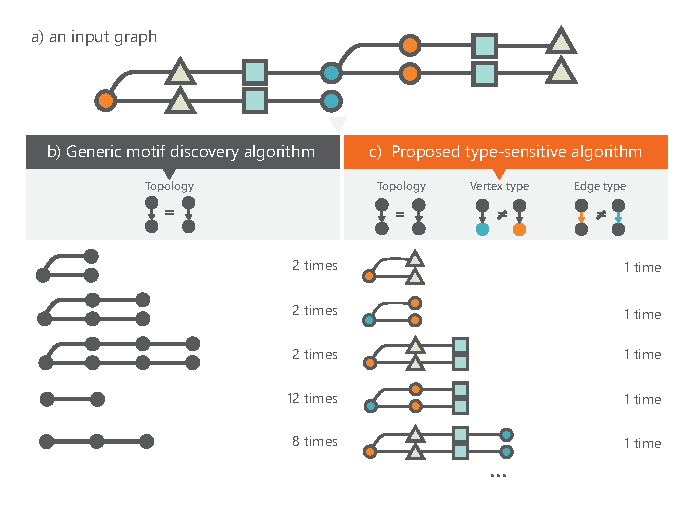
\includegraphics[width=.8\textwidth]{images/automacron/algorithm-differences.eps}
\caption{A) A graph, with typed nodes and edges, where different node types are mapped to different shapes and colours.
B) Generic motif discovery (or search) algorithms focus on topological differences.
C) Our motif extracting algorithm takes varying node/edge types into account, yielding semantically aware motif grouping.
}
\label{fig:new-algorithm-considerations}
\end{figure}

As shown in Table \ref{tab:motif-algorithms}, many motif search/discovery algorithms exist. 
Ribeiro \emph{et al.} \cite{ribeiro10}, Kashani \emph{et al.} \cite{kashani09} and Wong \emph{et al.} \cite{Wong:2012} published benchmarks detailing processing time for a subset of the algorithms in Table \ref{tab:motif-algorithms}.
As subgraph matching is fundamentally an \emph{NP}-complete problem, these algorithms are computationally intensive.
Wong \emph{et al.} report \emph{maVISTO} taking 14,000 seconds to find size three motifs in an \emph{E. Coli} network.
Comparing that to one second for \emph{FANMOD} to analyse the same network, one can see the huge variability in algorithm performance.
As the size of the target motifs grow, performance decreases.
Using the same \emph{E. Coli} network but searching for size 8 motifs, \emph{FANMOD} will need 9,000 seconds to finish the operation \cite{Wong:2012}.

In Table \ref{tab:motif-algorithms} the second column indicates whether the sampling is exact (enumerating all possible candidates) or estimated.
The third column indicates the maximum number of nodes in a motif the algorithm can handle.
The final column indicates whether the algorithm is focused on \emph{motif discovery} (finding repetitive patterns in a set of graphs), or \emph{motif search} (finding a given motif in a set of graphs). 
All algorithms focus on topological patterns in graphs only and do not consider the types of nodes and edges as a search constraint. 
However, the types, or semantic categories of nodes and edges are an interesting property in defining a macro.
There is a more semantically aware motif search algorithm implemented in \emph{VisComplete} \cite{scheideggerquerying2007,koopviscomplete:2008} that compares node labels and node order to predict the next step in a \emph{VisTrails} pipeline analysis over a larger corpus of pipelines.
However this algorithm is topologically less sensitive and provides no way to identify branch/merge events in a motif, or edge types.
A potentially useful algorithm for identifying suitable candidate macros should be type \emph{and} topology sensitive.
This chapter focuses on work to devise such an algorithm, offering additional advantages in computational performance and providing visual mappings with meaningful structural information. 

In our work, when considering whether a subset of steps in a given workflow is the same as another subset in the same or a different workflow, we must consider the semantics attached to each step (see Figure \ref{fig:new-algorithm-considerations}).
Consequently, the task of motif discovery and search is highly constrained by the types of nodes and edges.
Therefore, it is necessary, as well as advantageous, to develop specific motif extraction algorithms for workflow visualizations.
In addition, we propose a novel concept of partially automating the design of macro glyphs.
We consider the use of multi-resolution glyphs to depict macros at different levels of detail when a user interacts with the visualization, a technique referred to by Bederson and Hollan \cite{bedersonpad:1994} and later by Weaver \cite{weaverbuilding2004} as semantic zooming. 

% ==============================
\section{Motivation and System Overview}
\label{sec:Motivation}

Over the past two decades, Biology has benefited from entering the digital era, becoming a data intensive field.
Ancillary to this development, important efforts have been undertaken to preserve and curate digital artefacts in biology, including experimental workflows.
A workflow is a form of directed graph (digraph).
Scientists mainly rely on two types of workflow visualization: digraphs with text labelled boxes or glyph nodes.
The latter enables more compact visual representation than the former \cite{Maguire:2012:TVCG} allowing domain experts to perform their tasks such as error checking and comparison more quickly.
However, workflows can still be quite large and complex, containing many repeated subgraphs, which demand some effort for identification in ``flat'' representations.  
Hence, it is highly desirable to introduce macro representations in workflow visualizations, as both text-based and glyph-based workflow visualizations can benefit from macro-based visual compression.
Although experimental workflows in biology exhibit specific properties that are different from workflows in other disciplines, they often share some characteristics.
Almost all exhibit temporal ordering and most feature only acyclic digraph topologies.
We are therefore hopeful that our algorithm and experience can be transferred to workflow visualizations in other disciplines.

The domain experts involved in this work identified the following requirements: 

\vspace{-2mm}
\begin{enumerate}[itemsep=-1mm]
\item Given a number of workflows, can we obtain the most common patterns/motifs within those workflows?
\item For each motif, can we obtain the occurrence frequencies for that motif and information about which workflows they occur in?
\item Can we automatically create macro representations of those motifs, with the possibility of adding extra annotation to them?
\item Can motif patterns in a workflow be substituted by common macros to make the workflow more compact?
\end{enumerate}

\vspace{-1mm}
Depending on discipline and requirements, macros may be created by individuals based on their own knowledge about needs and usage.
However, such an individualised approach would be impractical if applied to the curation of large collections of experimental workflows as found in data repositories.
Yet, the availability of such data provides an opportunity for the computational identification of commonly occurring motifs in workflows.
The statistics of such motifs offer useful guidance to motif selection when defining macros.

To carry out this work, information was extracted from a curated resource currently holding over 22,000 experimental design workflows (ArrayExpress \cite{ArrayExpress::2012}).
We used a subset of this collection, comprising 9,670 workflows considered to be well-formed with respect to correct connectivity and semantic annotation.
This subset of workflows, available in the ISA-Tab format \cite{rocca-serra10, sansone12}, offers a good representation of experiment typology.
These ISA-Tab files were processed and transferred to a graph database, which provides an optimised environment for storing graph structures and a query language optimised for graph traversal \cite{batra12}. 
For this purpose, we selected \emph{Neo4j} \cite{Neo4J::2012} -- a freely available graph database providing a query language called Cypher, fast traversal algorithms and high scalability (up to several billions of nodes and edges on a single computer).

\begin{figure}[h!]
\centering
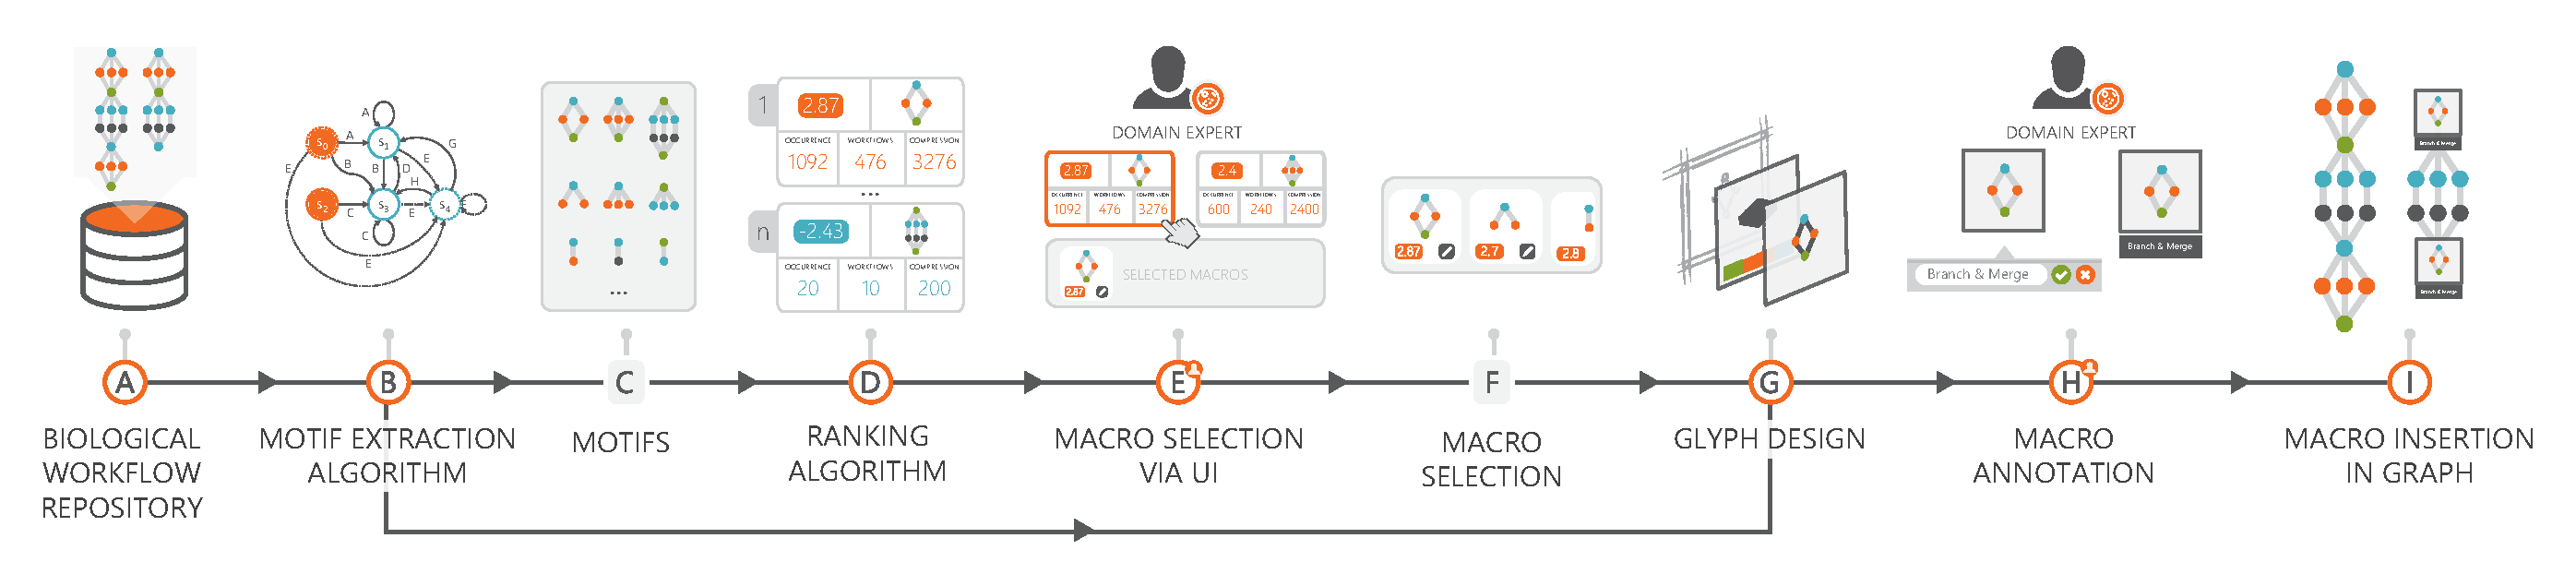
\includegraphics[width=\textwidth]{images/automacron/teaser}
\caption{An overview of the processes implemented in our system, AutoMacron, for compression of workflow visualizations. A) Biological workflows are imported from public repositories. B) The database of workflows is analyzed by our novel motif extraction algorithm that is sensitive to node/edge types and is built using a state-transition approach. C) The algorithm generates a large list of motifs. D) The motifs are ranked using metrics measuring their overall occurrence, scope of influence and compression potential. E) Based on the ordered recommendations by the system as well as their own knowledge, domain experts explore the space of motifs to identify suitable `macros'. F) A subset of motifs are selected for macro generation. G) A glyph is assigned to each macro automatically using a design pattern that utilizes the state output from the motif extraction algorithm. H) Domain experts are able to annotate macros with additional text labels. I) Macros can be inserted into the relevant workflows as a method for graph compression.}
\label{fig:automacron-teaser}
\end{figure}

Our system consists of a number of steps, as depicted in Figure \ref{fig:automacron-teaser}.
\begin{itemize}
\item \textbf{Step 1} (B, C, D) - we algorithmically scan all workflows in the collection and extract all valid subgraphs as candidate motifs.
The patterns and occurrence statistics of these motifs are recorded.
The definition of validity and the extraction algorithm will be detailed in Sections \ref{sec:Conditions} and \ref{sec:automacron_algorithm}.
\item \textbf{Step 2} (E, F) - we provide a user interface for domain experts to define macros by selecting motifs from an ordered list of candidates, based on the statistics computed as well as their domain knowledge about individual motifs and the context of their usage.
This will be discussed in detail in Section \ref{sec:Selection}.
\item \textbf{Step 3} (G, H) - we provide an automatic means for defining the pictogram of a macro by making use of the state transition information captured by the algorithm during the motif discovery phase.
In addition, each macro will normally be displayed with a text label, which is defined by the domain expert through the user interface.
The mechanism for automatic creation of a pictogram will be detailed in Section \ref{sec:Design}.
\item \textbf{Step 4} (I) - we created a tool to allow for substitution of frequent motifs with their macro counterparts in experimental workflows.
This functionality can be accessed via a standalone software package or through an API.
\end{itemize}

% ===============================
\section{From Motifs to Macros}
\label{sec:Motif}

Motif discovery and substitution in graphs typically consists of four processes. These are defined by Milo \etal \cite{Milo:2002} and Alon \cite{Alon:2007} as:

\vspace{-2mm}
\begin{enumerate}[itemsep=-1mm]
\item \emph{Subgraph Generation}: Scan each graph for all possible $n$-node subgraphs.
\item \emph{Motif Amalgamation}: Group together subgraphs that are topologically equivalent and generate a representative subgraph of each group (a motif).
\item \emph{Macro Selection}: Assign a significance value to each motif with respect to other motifs in the collection (for instance, by computing frequency of occurrence) and select the most significant motifs as macros.
\item \emph{Macro Substitution}: Search graphs for subgraphs that match with macros and replace them with that macro.
\end{enumerate}

\vspace{-1mm}
In applications such as biological network rendering, it can be safely assumed that subgraphs should be connected.
By contrast, in applications such as very-large-scale integration (VLSI) design, such a condition is sometimes relaxed, as macros are often used to group elements for a cost-effective spatial placement.
In general, the number of subgraphs can be rather large.
That is why many algorithms only deal with small subgraphs, such as the 4-node subgraphs studied in \cite{Milo:2002}.


\subsection{Candidate Macros in Workflows}
\label{sec:Conditions}
%
The workflows and macros considered in this work exhibit the following characteristics: 

\begin{enumerate}[itemsep=-1mm]
\item A workflow is an acyclic digraph.
\item A macro must consist of at least two nodes.
\item Macros are not only topologically sensitive, but also semantically sensitive. In other words, two subgraphs are said to be in the same motif group only if they are isomorphic and every pair of corresponding nodes (and edges) are of the same type.
\item It is not necessary to have a path between every pair of nodes in a motif.
\item For each node in a macro, there must exist a path from the macro's input node, and a path to the macro's output node.
\item Each macro must have a single input type and a single output type (including \emph{bundled} input and output).
\item A bundled input or output may contain any number of connection edges, but they must be of the same material type.
\item A macro may receive a bundled input converging from different preceding nodes and may deliver a bundled output branching off to different successive nodes.
\end{enumerate}

\begin{figure}[t!]
\centering
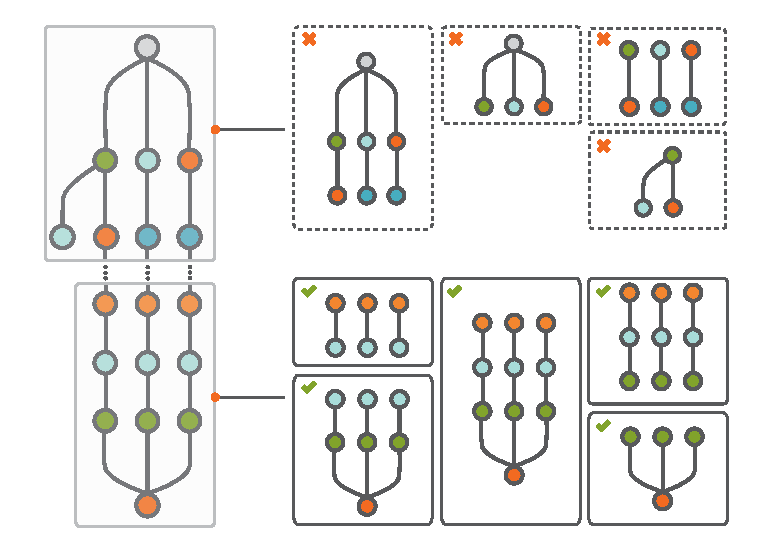
\includegraphics[scale=.6]{images/automacron/valid-invalid-motifs.eps}
\caption{In a workflow graph, some subgraphs can be considered as ``legitimate motifs'' while others cannot, depending on node type. Invalid motifs do not have the same output node type, as indicated by the differing colours. Conversely, valid motifs are those that have the same input and output node type.}
\vspace{-3mm}
\label{fig:Conditions}
\end{figure}


By relying on these characteristics we can significantly reduce the number of subgraphs and motifs to be extracted in the \emph{motif generation} stage of the algorithm.
Figure \ref{fig:Conditions} illustrates those subgraphs that are ``legitimate'' candidates and others that are ``illegitimate''.
In addition, owing to characteristic three described above, the \emph{Motif Amalgamation} and \emph{Macro Substitution} stages are much less onerous in comparison to subgraph matching based on topology only. 

% ---------------------------
\subsection{Motif Generation}
\label{sec:automacron_algorithm}
%
\begin{figure}[t!]
\centering
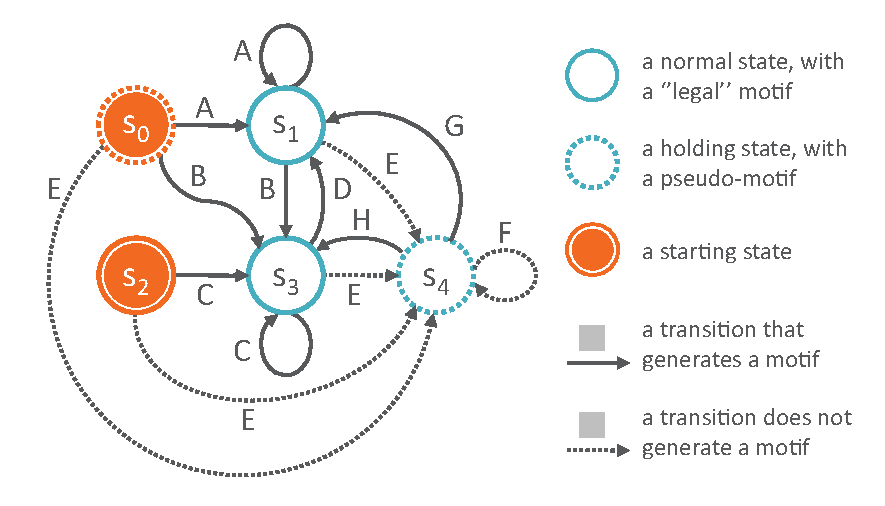
\includegraphics[width=.65\textwidth]{images/automacron/Transition.eps}
\caption{The full space of states and transitions between them encountered during motif generation.}
\label{fig:Transitions}
\end{figure}

\begin{figure*}[t!]
\centering
\begin{tabular}{@{}ccc@{}}
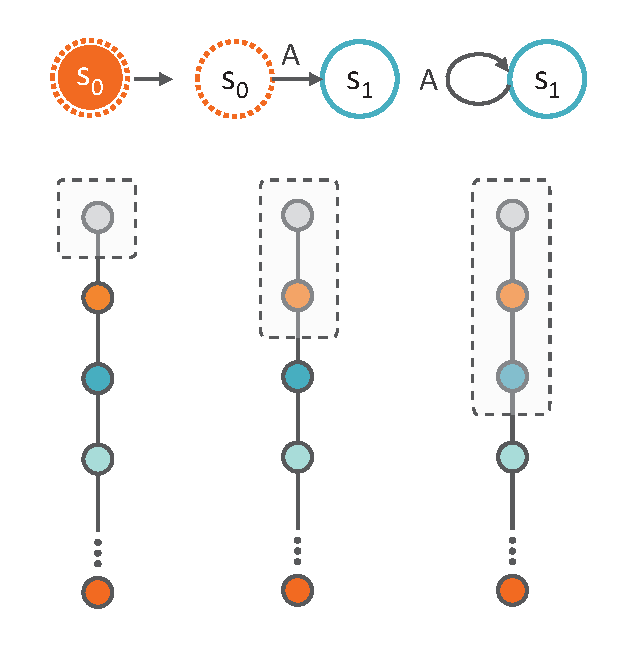
\includegraphics[width=37mm]{images/automacron/States1.eps}&
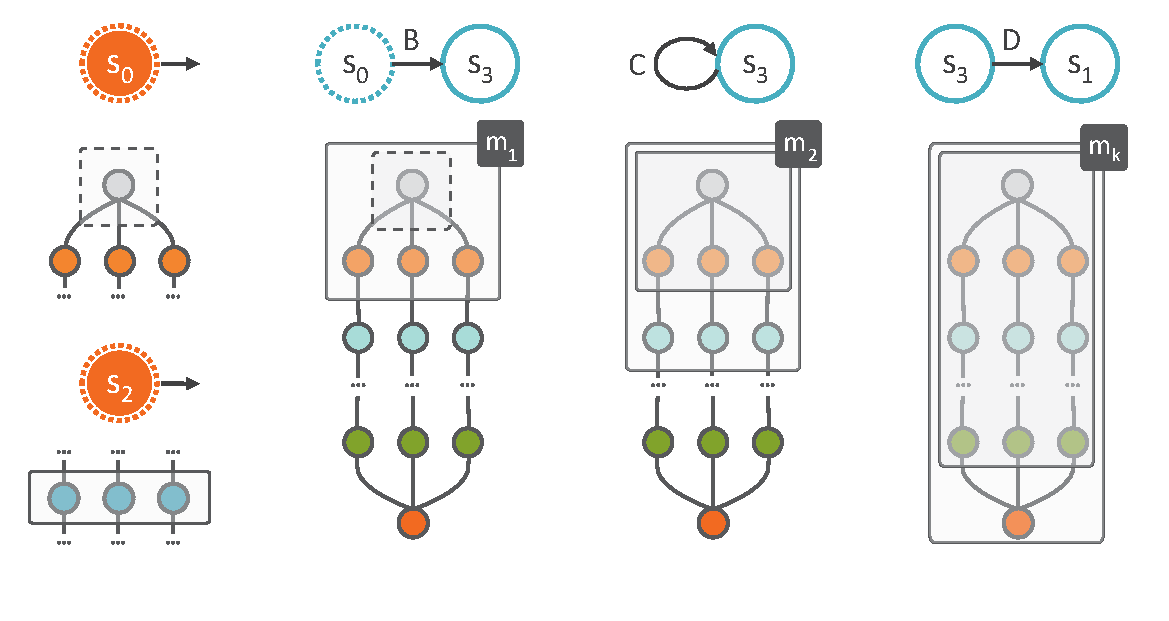
\includegraphics[height=37mm]{images/automacron/States2.pdf}&
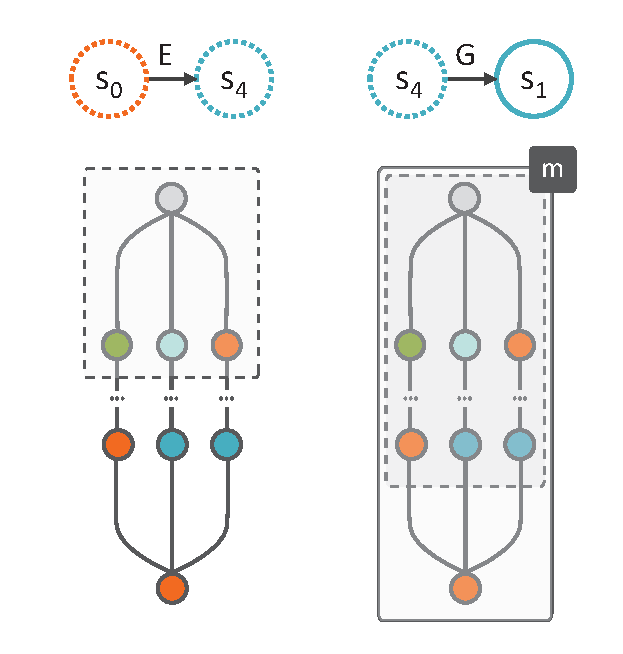
\includegraphics[height=37mm]{images/automacron/States3.eps}\\
A) singular branching & B) homogeneous branching & C) heterogeneous branching
\end{tabular}
\caption{Examples of state transitions with different rules. Homogeneous edges are depicted by using the same colour.}
\label{fig:States}
\end{figure*}

Owing to the aforementioned conditions that are specific to workflows, we could not make use of existing motif generation software and algorithms such as those surveyed in \cite{Wong:2012}.
A specialised motif generation algorithm was needed, and for that we adapted the widely accepted ``pattern growth'' approach \cite{Wong:2012}.
We describe the algorithm by evolving a state transition diagram as shown in Figure \ref{fig:Transitions}.

\noindent \textbf{Singular Branching (Rule A).}
%
As shown in Figure \ref{fig:States} A), the simplest workflow is perhaps a single path composed of $n$ different steps (\eg, experimental steps).
The algorithm can be activated from any node and will only move forward, following the flow of the work.
Since a single node cannot be a macro, the search will park at state $\mathsf{S}_0$ as illustrated in Figure \ref{fig:States} A), where the orange background indicates a starting state and the dotted outline implies that it is only a holding state and does not output a ``legitimate motif''.

When the algorithm encounters the next node $n_1$, it obtains the first ``legitimate motif'', $m_1 = \langle n_0 \rightarrow n_1 \rangle$, and moves to the state $\mathsf{S}_0$.
The edge is labelled with $A$ indicating that this follows rule \textbf{A}.
From $n_1$, the algorithm then encounters $n_2$, it outputs another motif $m_2 = \langle n_0 \rightarrow n_1 \rightarrow n_2 \rangle$, and remains at the same state.
For the workflow in Figure \ref{fig:States} A), this self-loop continues to generate motifs in growing sizes until the end of the path or the number of nodes in the motif reaches a predefined maximum. 

\noindent \textbf{Homogeneous Branching (Rules B, C, D).}
%
One extension of the singular branching case is multiple runs of the same sequence of steps, in parallel.
When the work flows forward, the same type of edges connect to the next set of nodes (see condition 7 in Section \ref{sec:Conditions}).

When an edge first branches to multiple nodes, as illustrated in Figure \ref{fig:Transitions}, the algorithm moves from state $\mathsf{S}_0$ or $\mathsf{S}_1$ to $\mathsf{S}_3$, following a transition of singular branching to bundled homogeneous branching.
This is referred to as rule \textbf{B}.
$\mathsf{S}_3$ indicates more than one edge is being bundled at this state and the number of edges may vary.

The algorithm will self-loop as long as the motif grows with such bundled edges.
Rule \textbf{C} indicates a transition within the state of homogeneous branching.
The number of edges in an edge bundle can change as long as there is more than one edge and they are of the same type.

When all bundled branches converge to a single node, the algorithm returns to state $\mathsf{S}_1$.
This transition is referred to as rule \textbf{D}.
Figure \ref{fig:States} B) shows three examples of applying rules \textbf{B}, \textbf{C} and \textbf{D} respectively.
Applying any of the three rules will result in a bigger motif than the previous one.

An additional state $\mathsf{S}_2$ is included for a scenario when the algorithm starts with a row of parallel nodes with bundled input and output.
We will discuss this scenario later in the context of reactivating the algorithm for bundled edges.

\noindent \textbf{Heterogeneous Branching (Rules E, F, G, H).}
%
Recall conditions 6 and 7 in Section \ref{sec:Conditions}: a macro must have a single input and single output and each can be bundled edges of the same material type.
When these two conditions are met, we can have heterogeneous flow within a macro.
This subset of rules is designed to ``grow'' this particular type of motif.

Rule \textbf{E} is applied when the algorithm first encounters an heterogeneous pattern.
This transition leads to a holding state $\mathsf{S}_4$ and it does not generate any motif.
In this state, all nodes scanned so far are grouped as an interim pseudo-motif and output edges are placed in an interim pseudo-bundle.

The interim state is maintained by a self-loop transition; \emph{i.e.}, rule \textbf{F} as long as the bundled edges remain heterogeneous.
When the edges in an interim pseudo-bundle finally converge to a single node or a set of nodes with homogeneous output edges, the algorithm can leave the holding state $\mathsf{S}_4$.
Rule \textbf{G} defines the transition to singular branching state $\mathsf{S}_1$, while rule \textbf{H} defines the homogeneous branching state $\mathsf{S}_3$.
Both rules will generate a new motif, which includes all nodes in the interim pseudo-motif and the newly encountered node(s).

\noindent \textbf{Termination and Reactivation.}
%
The algorithm strictly follows the breadth-first search strategy.
It may terminate in two situations:
(a) when the predefined maximum depth that a macro may be at is reached;
(b) when it encounters a node without an output edge (\emph{i.e.}, the termination point of a workflow).
The termination condition is tested in all states in Figure \ref{fig:Transitions}.

It is necessary to reactivate the algorithm by choosing each of the different nodes in a workflow as a starting node at state $\textsf{S}_0$.
In addition, each bundle of edges of the same material type can also be a starting point at $\textsf{S}_2$.
Although theoretically appropriate, invoking the algorithm recursively from a starting node of a workflow proved not to be feasible in practice.
We therefore made use of a queue, which initially contains all nodes in a workflow.
We fetch nodes from the queue one at time to invoke the algorithm from $\textsf{S}_0$.
Every time the algorithm reaches state $\textsf{S}_3$, we have a set of homogeneous nodes that were just encountered (\eg, $[n_{1a}, n_{1b}, n_{1c}]$ in Figure \ref{fig:States} B)).
We store all $k$-node subsets of such a set ($k = 2, 3, \ldots$) in a list.
When we finish with all individual nodes in the queue, we sort the list and remove redundant subsets.
We then invoke the algorithm with the sorted and cleaned list from $\textsf{S}_2$.
Note that each subset in the list is a ``legitimate motif'', hence $\textsf{S}_2$ is not a holding state.


% I have to add in the stuff from my meeting with Min here further qualifying why we devised our own algorithm. 

\noindent \textbf{Performance.} To evaluate the performance of the algorithm, we tested it against nine graphs representing biological workflows of varying sizes on a MacBook Pro with a 2.53GHz Intel Core i5 CPU and 8GB RAM.

\begin{figure}[t!]
\centering
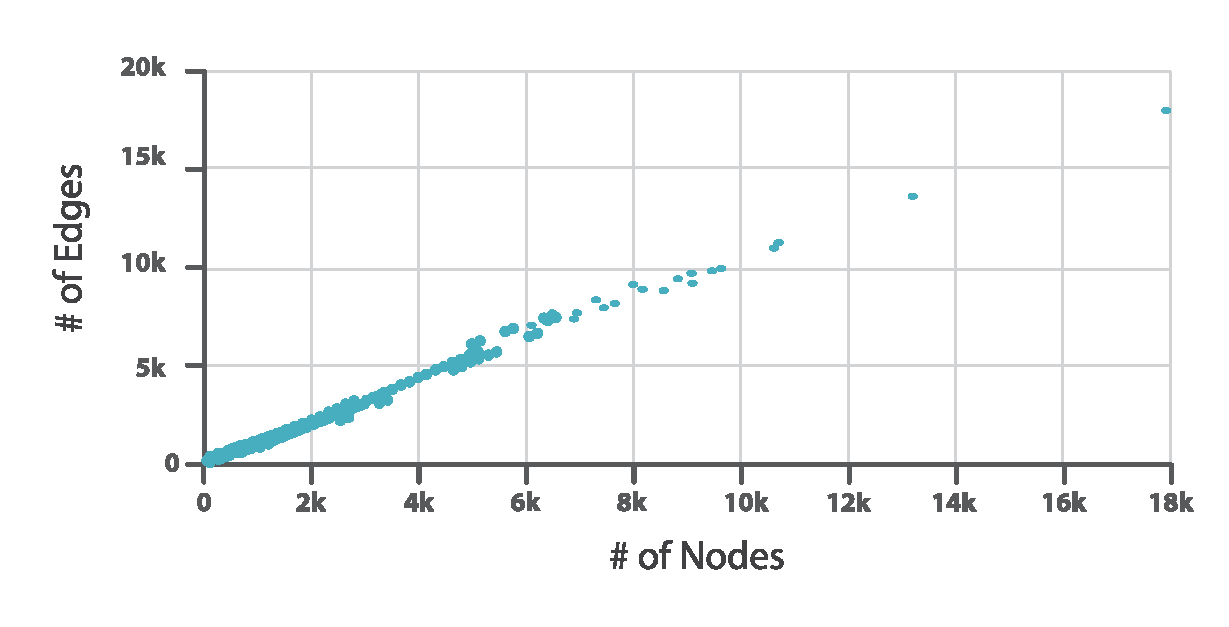
\includegraphics[width=.75\textwidth]{images/automacron/workflow-size.eps}
\caption{Scatter plot showing the distribution of workflows (each depicted as a point) as node count versus edge count.}
\vspace{-4mm}
\label{fig:workflow-size}
\end{figure}


The nine graphs were divided into three groups, three small, three medium and three large, based on their node and edge counts.
Figure \ref{fig:workflow-size} shows the distribution of workflows in our collection in terms of nodes ($x$-axis) and edges ($y$-axis).
93\% of all workflows have a node count below 1,000 and the average number of nodes per workflow is approximately 322.
Given these statistics, we define \emph{small} as 200 nodes or below (covering 58\% of workflows); \emph{medium} between 201 and 600 nodes (covering a further 28\% of workflows); and \emph{large} over 601 nodes (covering the remaining 14\%). 

\begin{table}[t!]
\centering
\vspace{1mm}
\scalebox{0.8}{
\begin{tabular}{|l|r|r|r|r|r|}
\hline
\textbf{Graph Size} & \multicolumn{1}{l|}{\textbf{Motif Depth}} & \multicolumn{1}{l|}{\textbf{G1}} & \multicolumn{1}{l|}{\textbf{G2}} & \multicolumn{1}{l|}{\textbf{G3}} & \multicolumn{1}{l|}{\textbf{Seconds}} \\ \hline
 \multicolumn{ 1}{|l|}{} & 3 & 0.018 & 0.017 & 0.024 & 0.02 \\ \cline{ 2- 6}
\multicolumn{ 1}{|l|}{} & 4 & 0.034 & 0.026 & 0.025 & 0.03 \\ \cline{ 2- 6}
\multicolumn{ 1}{|l|}{} & 5 & 0.048 & 0.038 & 0.042 & 0.04 \\ \cline{ 2- 6}
\multicolumn{ 1}{|l|}{} & 6 & 0.059 & 0.041 & 0.046 & 0.05 \\ \cline{ 2- 6}
\multicolumn{ 1}{|l|}{Small} & 7 & 0.075 & 0.049 & 0.049 & 0.06 \\ \cline{ 2- 6}
\multicolumn{ 1}{|l|}{} & 8 & 0.086 & 0.063 & 0.06 & 0.07 \\ \cline{ 2- 6}
\multicolumn{ 1}{|l|}{} & 9 & 0.095 & 0.064 & 0.062 & 0.07 \\ \cline{ 2- 6}
\multicolumn{ 1}{|l|}{} & 10 & 0.106 & 0.069 & 0.072 & 0.08 \\ \hline
\multicolumn{ 1}{|l|}{} & 3 & 0.153 & 0.065 & 0.056 & 0.09 \\ \cline{ 2- 6}
\multicolumn{ 1}{|l|}{} & 4 & 0.212 & 0.097 & 0.085 & 0.13 \\ \cline{ 2- 6}
\multicolumn{ 1}{|l|}{} & 5 & 0.24 & 0.13 & 0.115 & 0.16 \\ \cline{ 2- 6}
\multicolumn{ 1}{|l|}{} & 6 & 0.293 & 0.161 & 0.138 & 0.2 \\ \cline{ 2- 6}
\multicolumn{ 1}{|l|}{Medium} & 7 & 0.343 & 0.189 & 0.159 & 0.23 \\ \cline{ 2- 6}
\multicolumn{ 1}{|l|}{} & 8 & 0.389 & 0.219 & 0.178 & 0.26 \\ \cline{ 2- 6}
\multicolumn{ 1}{|l|}{} & 9 & 0.429 & 0.241 & 0.183 & 0.28 \\ \cline{ 2- 6}
\multicolumn{ 1}{|l|}{} & 10 & 0.477 & 0.287 & 0.192 & 0.32 \\ \hline
\multicolumn{ 1}{|l|}{} & 3 & 0.296 & 0.756 & 0.354 & 0.47 \\ \cline{ 2- 6}
\multicolumn{ 1}{|l|}{} & 4 & 0.393 & 1.062 & 0.45 & 0.64 \\ \cline{ 2- 6}
\multicolumn{ 1}{|l|}{} & 5 & 0.652 & 1.309 & 0.414 & 0.79 \\ \cline{ 2- 6}
\multicolumn{ 1}{|l|}{} & 6 & 0.632 & 1.528 & 0.42 & 0.86 \\ \cline{ 2- 6}
\multicolumn{ 1}{|l|}{Large} & 7 & 0.75 & 1.829 & 0.341 & 0.97 \\ \cline{ 2- 6}
\multicolumn{ 1}{|l|}{} & 8 & 0.809 & 2.028 & 0.396 & 1.08 \\ \cline{ 2- 6}
\multicolumn{ 1}{|l|}{} & 9 & 0.889 & 2.287 & 0.528 & 1.23 \\ \cline{ 2- 6}
\multicolumn{ 1}{|l|}{} & 10 & 1.047 & 2.489 & 0.604 & 1.38 \\ \hline
\end{tabular}
}
\caption{Performance of our motif-finding algorithm on graphs of varying size and at a range of search depths. 
Averages (last column) are taken across three graphs G1, G2, and G3 in each category. 
For each graph at each depth, the recorded time was the average time over five runs. A more detailed table is available in the supplementary materials.}
\label{tab:performance}
\end{table}

\begin{figure}[ht!]
\centering
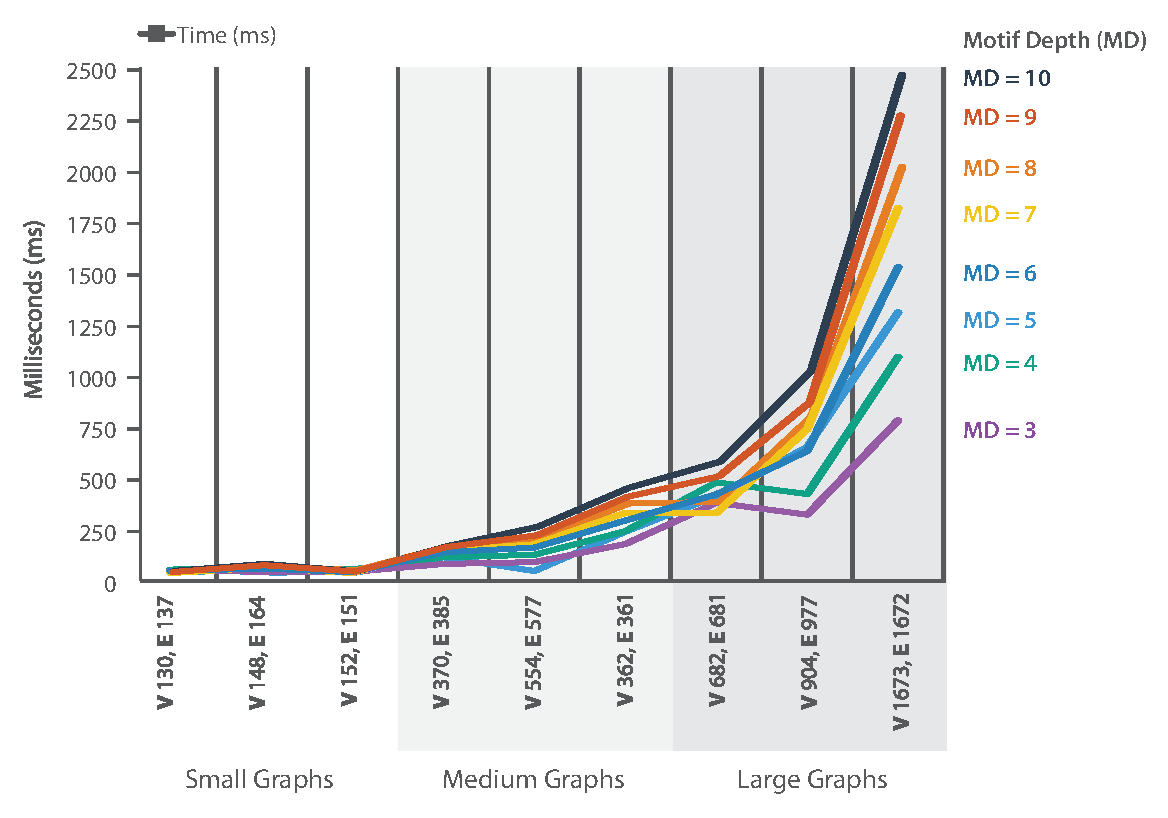
\includegraphics[width=.8\textwidth]{images/automacron/results_graph}
\caption{Overview of our motif finding algorithm's performance at different motif depth cut-offs across small, medium, and large graphs.}
\label{fig:eval_results_graph}
\end{figure}

For each of the nine selected graphs, motifs between a depth of three and ten were searched for, with each search repeated five times to account for any variability.
Table \ref{tab:performance} gives the runtime (in seconds) of applying our algorithm to the nine test graphs.
Results are also summarised in Figure \ref{fig:eval_results_graph}. 
The runtime is scalable to our collection of some 10,000 workflows, as the algorithm runs as a batch process.
It also shows that the speed of our motif finding algorithm compares favourably the current best general purpose motif finding algorithms.

Our algorithm search space differs from the general purpose algorithms listed in Table \ref{tab:motif-algorithms}, since we have introduced specific constraints on motif structure, taking into account the notion of node/edge types.
Nevertheless, we could have theoretically used a two-stage method, by first using a general-purpose algorithm to identity an initial list of motifs, then filtering out those motifs that do not meet our requirements.
Since our algorithm is generally faster than these general purpose algorithms, plus the computation to infer back the node/edge type is potentially large, there is no advantage to using this two-stage approach.


% -------------------------------------
\subsection{Selecting Macros from Candidate Macros}
\label{sec:Selection}

\begin{figure*}[t!]
\centering
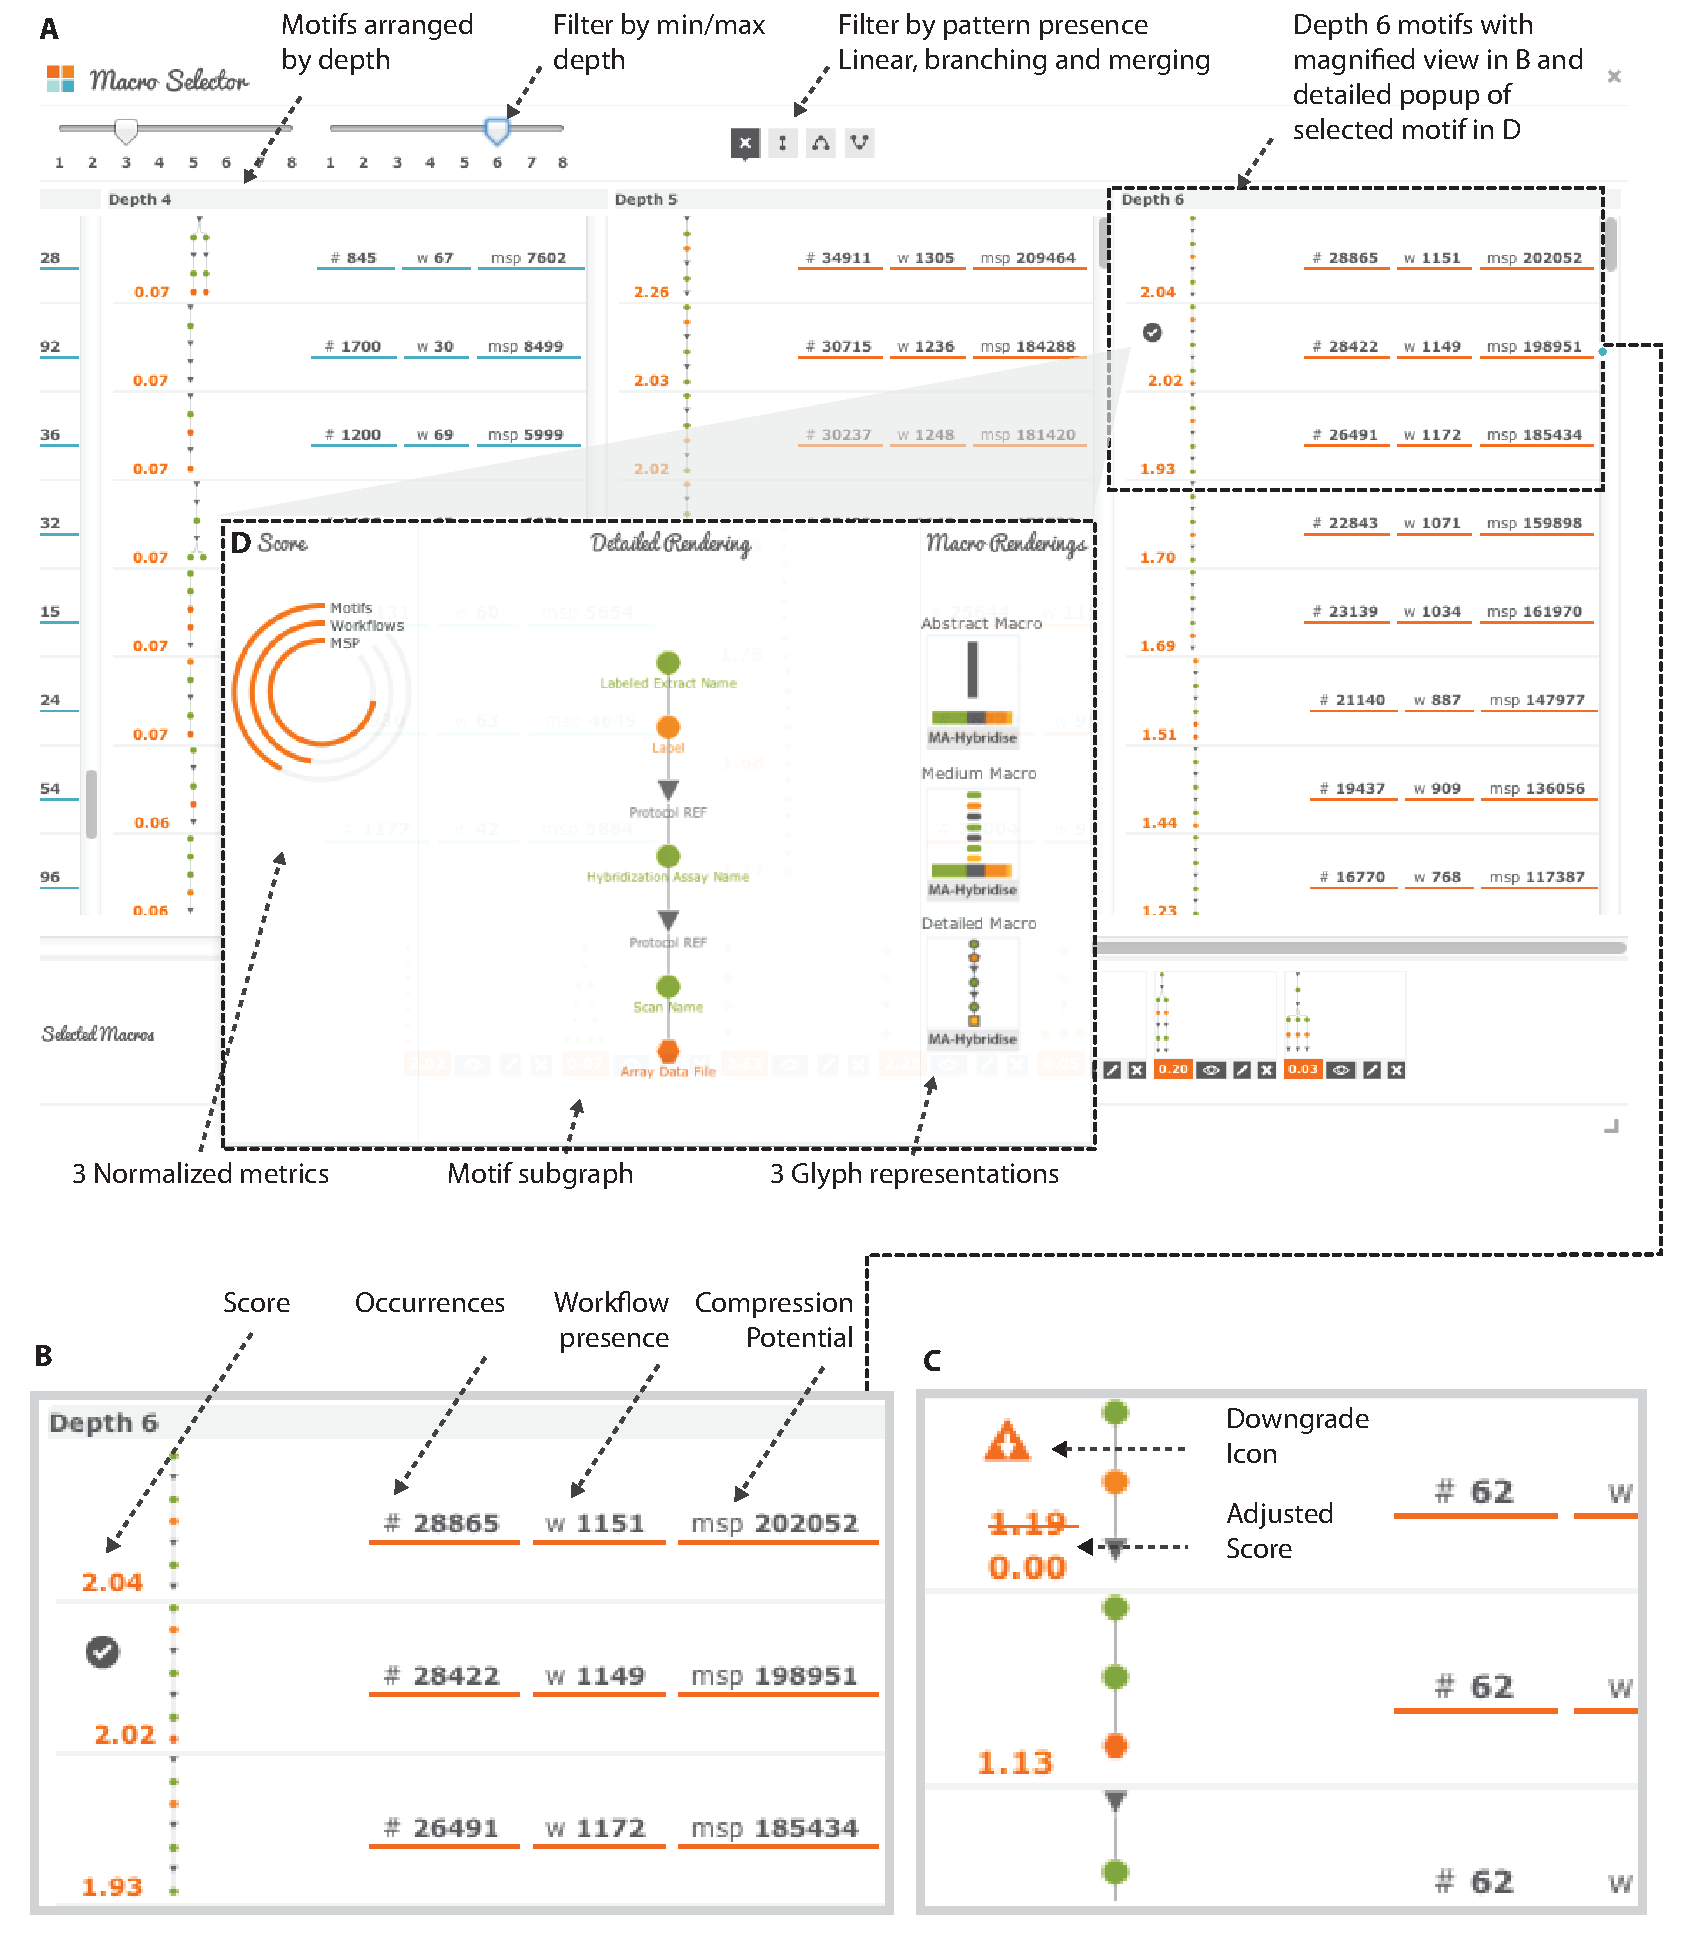
\includegraphics[width=\textwidth]{images/automacron/motif-selection-09}
\caption{AutoMacron provides a user interface (A) for domain experts to select macros from a list of computed motifs.
As shown in the detailed view in (B), the overall score determines the order of motifs in the list.
% The scores are color-coded with higher values (in orange) and lower values (in blue). 
The three indicators are shown in unnormalized form in order to be semantically meaningful.
The detail view (C) shows an example where a score is adjusted dynamically when a motif encompassing other motifs is selected.
(D) shows a pop-up window for a specific macro, detailing its subgraph and three automatically generated pictograms for different levels of details in visualization.}
\label{fig:motif-selection}
\end{figure*}

Given a list of motifs extracted using the algorithm in Section \ref{sec:Algorithm}, we can categorise them into individual groups.
Motifs in each group share the same subgraph topology, and the same set of nodes and edges in terms of their numbers and types.
Each motif group thus becomes a candidate macro.
It is important to emphasise that selecting macros from macro candidates requires a fair amount of knowledge about biology, biological experiments, and the uses of workflows.
In some cases, other information, such as the time when and context in which certain motifs appear frequently, may also feature in the selection process.
Therefore, it is not sensible to make this selection process fully automatic.
In this work, we provide a user interface to assist domain experts in selecting macros from a large list of candidates.

Following the advice of domain experts specialised in biological data curation, we understood the essential requirement for such a user interface is to provide key indicators for each macro candidate $g_i$, including the depth of its subgraph, $A_d(g_i)$, the total number of its occurrences in the data repository, $A_t(g_i)$, the number of workflows that contain it, $A_w(g_i)$, and its compression power $A_c(g_i)$.
For each indicator, normally the higher value the indicator has, the more selectable the candidate is.
However, when the comparison is not clear cut across different indicators, the domain experts will have to make an informed decision based on all the indicators as well as their tacit knowledge about the macro candidate (\eg, biological semantics, importance in science, expected future usage).
As shown in Figure \ref{fig:motif-selection}B, the user interface displays each candidate with these indicators.
The candidates are organised into columns, each representing a specific depth of the subgraphs in all macro candidates. 
Each candidate is shown with the basic pattern along with three indicators, $A_t, A_w, A_c$.
The detailed structure of each macro candidate can be viewed on demand by using mouse interaction.

In order to help domain experts examine a large number of candidates speedily, we sort macros candidates in each column by a ranking score, allowing domain experts to inspect the most promising candidate first.
The ranking score is based on indicator $A_t$, $A_w$, and $A_c$.

\noindent \textbf{Indicator 1: Occurrences in the data repository.} Indicator $A_t$ returns the total number of times a motif has occurred across the entire database of workflows.
It emphasises the importance in selecting motifs that are highly used, inferring their functional importance. 

\noindent \textbf{Indicator 2: Workflow presence.} Indicator $A_w$ returns the total number of workflows in which a motif has appeared.
This provides a measure of how widely a motif is used across different biological experiments, counterbalancing the possible distortion in situations where a motif is heavily used in a relatively small number of workflows. 

\noindent \textbf{Indicator 3: Compression Potential.} Indicator $A_c$ is calculated by first subtracting the number of nodes in the motif ($A_n$) by 1, since these nodes will be replaced by a single macro node, and then multiplying by its occurrence ($A_t$).
It is written as $A_c(g_i) = (A_n(g_i) - 1) * A_t(g_i)$.

For each of these three indicators, we map it to a fixed range $[-1, 1]$ using a linear mapping based on the min-max range of each indicator, yielding three normalised metrics $M_1$, $M_2$, and $M_3$.
These are combined into a single ranking score using a weighted average as:
\[
S(g_i) = \sum_{k=1}^3 \omega_k M_k(g_i)
\]
\noindent where $\omega_k$ are three weights defined by users.
Our system makes no assumptions about the merits of one indicator over another, so the default weights are set to one.
We chose to have the score $S(g_i)$ in the range of $[-3, 3]$, as it helps domain experts to connect the score back to the three indicators.

Figure \ref{fig:motif-selection} shows a screenshot of the user interface on the left (A), and two detailed views with annotation on the right (B, C).
A domain expert normally examines macro candidates with the largest depth value (the rightmost column) first.
Once a motif, $\mathcal{M}$, is selected, it may affect the current results returned by the indicators.
As such a motif, $\mathcal{M}$, may contain many other candidate motifs as subgraphs. It is important for the domain expert to be aware of the impact of this decision on those candidate motifs yet to be examined.
The system thus updates the indicators of all those candidate motifs included in $\mathcal{M}$.
Instead of modifying $A_t$ and $A_w$ directly, the system shows a corrected score calculated by considering the new values for $A_t$, $A_w$ and $A_c$, implying the difference if all $\mathcal{M}$ were to be removed from the repository.

% ====================
\section{Macro Design}
\label{sec:Design}

\begin{figure*}[t!]
\centering
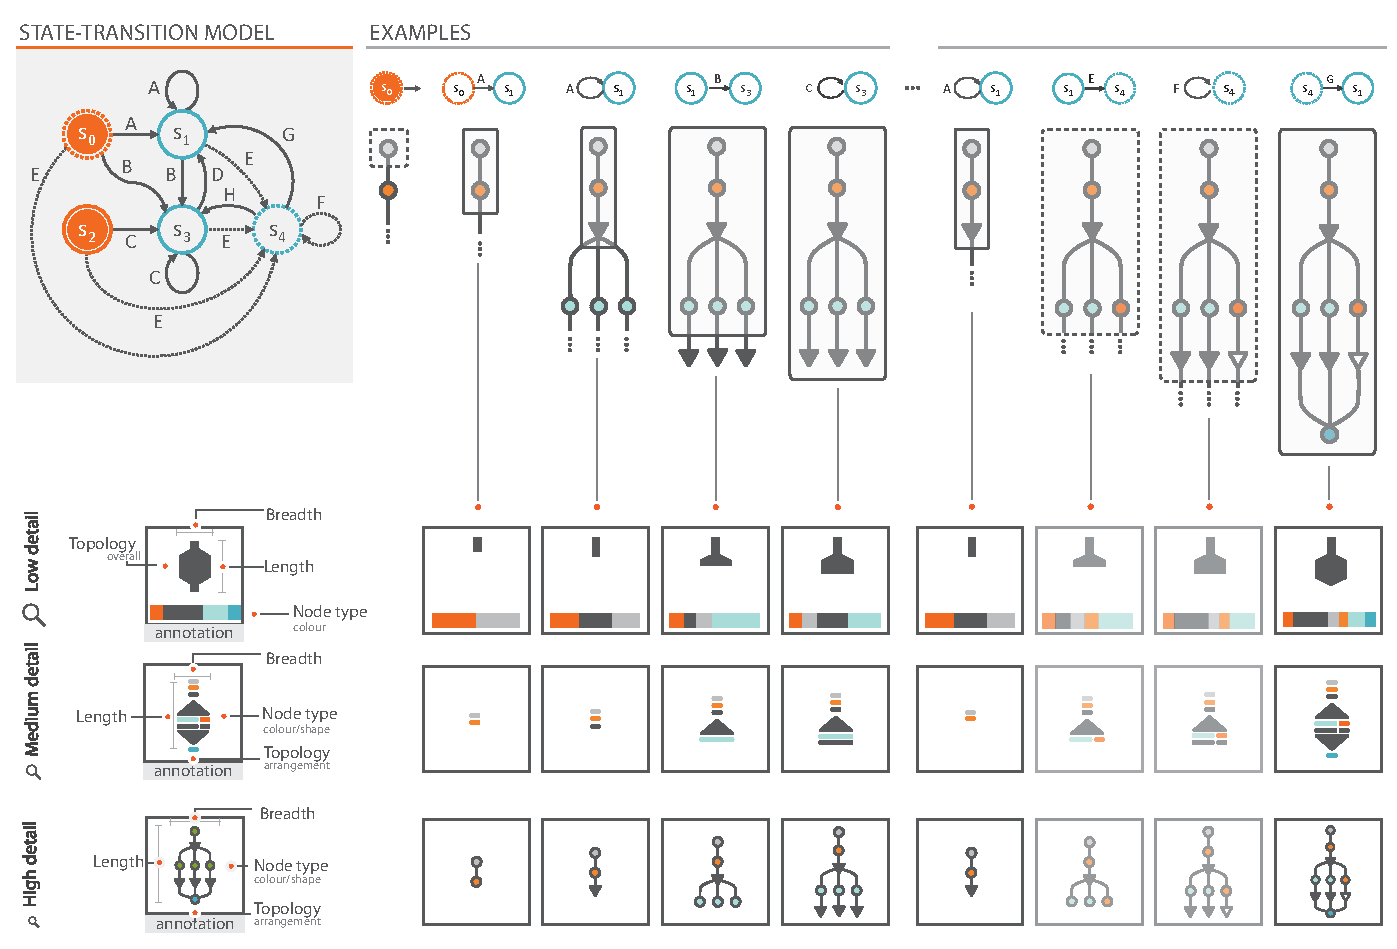
\includegraphics[width=\textwidth]{images/automacron/macro-design-options.pdf}
\caption{From left to right: automatic generation of a micro pictogram based on the state transitions encountered.
The lower three rows: Three design options for representing macros.}
\label{fig:design-options}
\vspace{-3mm}
\end{figure*}

Having obtained a collection of motifs suitable for use as macros within our corpus of workflows, we now have the task of designing their visual representation.
It is important to keep the users in mind and ensure that the design reflects what a typical user, in our case a biologist, would expect to find in a macro. 
We consulted domain experts as to the visual elements that users considered the most important to view.
A number of attributes were identified and are listed below in order of importance:

\vspace{-2mm}
\begin{enumerate}[itemsep=-1mm]
\item an impression of topology/structure within a macro (\eg, it may be an entirely linear path, a set of parallel paths, or it may contain branch/merge events);
\item an impression of types of nodes in a macro (\eg, the overarching theme of the macro);
\item textual description, (\emph{i.e.}, additional annotation to provide concrete semantic meaning and help in understanding);
\item an impression of density within a macro, (\emph{i.e.}, the size of the corresponding subgraph).
\end{enumerate} 

\vspace{-1mm}
Given the attributes listed above, we devised three design options, as illustrated in Figure \ref{fig:design-options}, for creating pictograms.
These pictograms are created automatically based on the states encountered when the motif is found by the motif generation algorithm in Section \ref{sec:Algorithm}.
When the algorithm moves from one state to another, the pictogram grows by adding a new visual component reflecting the subgraph pattern just encountered.
We provide three alternative designs for each macro.
The first option is pixel-based, the second is shape-based and the third is a miniature version of the subgraph.
All three design options are stored as vector graphics, so they are suitable for multi-scale display, for example, through zooming operations.
Textual descriptions of the macros are always provided by experts.


Figure \ref{fig:motif-selection}(D) shows a pop-up window with a detailed view of a macro, and the three design options.
The users can choose to have a fixed design for the macro, or have a multi-scale variation according to the level of detail at which a user is viewing the workflow.

\noindent\textbf{Overview/Low detail}. At the overview level, the fine-grained details of the workflow (\emph{e.g.,} lines) utilise visual channels occupying a high spatial frequency.
It is more effective for nodes in a graph to occupy low spatial frequencies, which will be distinguishable by a user.
The pixel-based design option enables users to use visual channels that are visible and roughly distinguishable in low spatial frequencies.
Although individual nodes and edges are not visible, the user can still gain a rough impression about the topology and node types. 

\noindent\textbf{Medium detail}. At medium detail, users should be able to see more information through the shape-based design.
The major steps from input to output (\emph{i.e.}, following the state transitions) become more distinguishable.
Each horizontal segment of the pictogram is coloured by node type, branching and merging is shown with triangles of mirrored directionality, and heterogeneity of nodes is depicted in separated tracks of differing colours. 

\noindent \textbf{High detail}. When a user zooms into a small region of the visualization, a miniature version of the subgraph becomes available, showing details of the topology and node types. This representation has a lot of high spatial frequency information and is only suitable for detailed examination in close up views.

\section{Software Implementation and Use}

To demonstrate our approach, we developed an open-source Java tool named \emph{AutoMacron} that may be used in two modes: 1) standalone for those wishing to discover common motifs in a database of graphs; and 2) as an API for those wishing to integrate the utilities for motif discovery into their own software.
The software provides the following functionalities:

\vspace{-2mm}
\begin{enumerate}[itemsep=-1mm]
\item Load files that have a handler (\emph{e.g.,} ISA-Tab in our use case) into a graph database;
\item Analysis of all graphs in the database instance to determine the dominant motifs;
\item Allow for selection of macros from the pool of over-represented motifs found by the algorithm;
\item Visualise graphs both in uncompressed/compressed representations, and/or export those graphs in GraphML format for visualization in other environments; 
\item Render differing images depending on the zoom level (semantic zooming \cite{bedersonpad:1994,weaverbuilding2004}). For this, we have extended the Prefuse visualization library \cite{heer05}.
\item Allow for search of a graph database for a user-defined semantically-annotated motif;
\item Export macros for use in other software.
\end{enumerate}

\vspace{-1mm}
Using AutoMacron, over 12,000 valid motifs were found in a collection of 9,670 existing workflows from ArrayExpress. From that set, those motifs scoring below zero with the aforementioned aggregated score $S(g_i)$ were removed from consideration leaving just over 400 candidates. 

Further examination of these candidates was conducted by domain experts using the macro selection utility shown in Figure \ref{fig:motif-selection}.
Examination is aided through both presentation of the metrics and ``live'' highlighting of motif representations as they occur in the original graph representation.
Following the manual selection of 30 of these macros, the domain experts labelled each macro with a textual description, making the corresponding glyphs more meaningful and identifiable. These macros could then be used to substitute the more complex representations in the original graph in an effort to compress the representation.

% talk about insertion in to ISAcreator. Graph database assistance etc. Use of macros can be presented in an easily accessible tool. 

\begin{figure*}[ht!]
\centering
\includegraphics[width=\textwidth]{images/automacron/isacreator-48.eps}
\caption{A) A typical workflow, where a 4-node motif is selected as a macro using AutoMacron. (B) A screenshot of  ISAcreator, which using the AutoMacron API can replace each occurrence of the 4-node motif with its macro representation.}
\vspace{-1mm}
\label{fig:isacreator}
\end{figure*}

Aside from the dedicated \emph{AutoMacron} tool, the motif finding functionalities have been incorporated into ISAcreator, which is a tool used by domain scientists to annotate and curate biological experiment workflows and other necessary documentation. As shown in Figure \ref{fig:isacreator}, the user is given the option to compress an experiment workflow using the macros selected by domain experts for biological data curation. 

\section{Evaluation}

Aided by direct collaboration and regular interaction with domain experts, development of the software followed an evolutionary prototyping process whereby users evaluated the prototype at every major stage of the development. For each prototype users contributed their feedback to the software and algorithm outputs. 

In this section, we summarise the feedback given from the last iteration where we performed the following: 1) analysis of the performance of the algorithm presented in this work in comparison with that of the best existing (and available) algorithm; and 2) observation of how the software met the initial requirements as identified in Section \ref{sec:Motivation} by interviewing expert users.

\subsection{Evaluation Against Existing Algorithms}

\begin{figure*}[ht!]
\centering
\includegraphics[width=.8\textwidth]{images/automacron/evaluation.eps}
\caption{A) A simple experimental graph visualized using the software from Maguire \emph{et al.} \cite{Maguire:2012:TVCG}. In this example, we are showing a specific pattern and how that pattern is represented in both FANMOD and AutoMacron. B) HTML Output for 4-node motifs from FANMOD's analysis identifies 5 motifs with 4 nodes. 2 are incorrect (highlighted in orange) according to our rule set in Section \ref{sec:Conditions}. C) HTML output from AutoMacron's analysis which identifies all 50 motifs. We have highlighted the specific motif being searched for (in blue) matching the highlight pattern in A and B, and show the other serial 4 node motifs (highlighted in grey) that would erroneously be considered the same had it not been for preserved semantics of nodes and edges.}
\vspace{-4mm}
\label{fig:automacron-evaluation}
\end{figure*}

We wished to test the performance of the best in class in existing algorithms with that of the algorithm presented in this work, not necessarily just in speed, but also in what was found and how that compared with domain experts' expectations.
We compared the performance of FANMOD \cite{wernicke06} and the algorithm presented in this work in an attempt to discover which motifs could be found and how they related to the expectations of domain experts.

First, we ran a simple test graph through FANMOD, to detect three, four, five, six, seven, and eight node graphs.
In FANMOD, there is a requirement to run each analysis separately, searching for size 8 node subgraphs does not yield all three to eight node subgraphs.
Figure \ref{fig:automacron-evaluation}B shows the output of a four node motif analysis and highlights FANMODs motif discovery match for a pattern highlighted in Figure \ref{fig:automacron-evaluation}A.
As aforementioned, there is no notion of node or edge type, therefore all four node graphs with the same serial topology will be the same, even though they represent entirely different concepts.
Additionally, FANMOD, typical of the existing class of algorithms, returns invalid results with respect to our definition of a motif as defined in Section \ref{sec:Conditions}.

Following this, we ran the same graph through AutoMacron to generate motifs up to depth eight. Note that FANMODs restriction is on node number (up to eight), whereas our algorithm can have potentially hundreds of nodes at depth eight. Figure \ref{fig:automacron-evaluation} C shows the HTML output from AutoMacron's analysis. The highlighted motif corresponds to those highlighted in Figures \ref{fig:automacron-evaluation}A and B, we magnify the motif to show how our algorithm identifies the exact pattern with topology, node, and edge type preserved.

Finally, we had the domain experts who inspected the graph manually and extracted the motifs they would expect the algorithm to find.
We compared what FANMOD and AutoMacron found with what the user expected.
Our summary results are shown in table \ref{tab:evaluation} with all analysis outputs available at \url{https://bitbucket.org/eamonnmag/automacron-evaluation}.

\begin{table}[!t]
\centering
\vspace{2mm}
\scalebox{1}{
  \begin{tabular}{|c|c|c|c|c|c|c|}
  \hline
  \textbf{Source} & \textbf{Motif Id.} & \textbf{Valid Motifs} & \textbf{Acc} & \textbf{MIdent} & \textbf{UIdent} & \textbf{Time (ms)} \\ \hline
  Domain Experts & 6 & 6 & 100\% & n/a & n/a & n/a \\ \hline
  FANMOD & 73 & 19 & 26\% & 4/19 (21\%) & 5/6 (83\%) & 1030*  \\ \hline
  AutoMacron & 50 & 50 & 100\% & 49/50 (98\%) & 6/6 100\% & 119 \\ \hline
  \end{tabular}
}
\caption{Results of motif identification by the domain experts, FANMOD and AutoMacron. Analysis included: \textbf{MIdent} - the ability of the domain experts to identify motif pictograms generated by the algorithms and match them to the original graph; and \textbf{UIdent} -  the percentage of motifs found by the algorithm with respect to the number identified manually by the domain expert.
Timings for how long it took the domain experts to find motifs was not recorded, hence it's not applicable (n/a) tag.}
\label{tab:evaluation}
\end{table}

The results show that AutoMacron identifies less macros that FANMOD, however if one was to consider all the invalid motifs AutoMacron filters out due to incompatibility with our rule set (see Section \ref{sec:Conditions}), AutoMacron would have reported many more. When we consider just the ``valid'' motifs, AutoMacron has many more than FANMOD (fifty compared with nineteen for FANMOD). 
This is as a direct result of the semantics added by AutoMacron. To illustrate, consider a simple two node directed subgraph ($v \rightarrow v$) with three possible node types ($n$), AutoMacron could theoretically identify $n(n-1)$ different motifs whereas FANMOD and other algorithms already listed here could only identify one.
Figures \ref{fig:automacron-evaluation} B and C show for instance how one 4-node motif found in FANMOD maps to five potential, but only one correct motif in AutoMacron. Overall both algorithms identified the majority of motifs expected by the user, not unexpected considering both mechanisms are exhaustive, however FANMOD struggled when it came to identifying the larger motifs, due to the node limit of eight, hence its UIdent value of 83\%. 

The user was also asked to identify motifs based solely on the pictograms representing topology (macros) output from each program.
In 98\% of occasions, the user could identify AutoMacron motifs, aided by both colour coding and better topological arrangement.
With FANMOD however, the user was able to decode 21\% of the outputs. 

\subsection{Evaluation Against User Requirements}
%
The algorithm and tool were tested by two biologists from the University of Oxford who were also authors on the resulting paper (Dr. Susanna-Assunta Sansone and Dr. Philippe Rocca-Serra).
Our tests served to determine how the software has met the four requirements identified in Section \ref{sec:Motivation}.
For each requirement, we summarise their feedback below.

\vspace{-2mm}
\begin{enumerate}[itemsep=-1mm]
\item Given a number of workflows, can we obtain the most common patterns/motifs within those workflows?
  
    \emph{We tested AutoMacron on nearly 10,000 workflows, the software returned an abundance of motifs that were sorted by a score. The filtering tools helped us in finding motifs with specific topological events.}
  
\item For each motif, can we obtain the occurrence frequencies for that motif and information about which workflows they occur in?
  
    \emph{For each motif reported by the software, we were able to recover statistics about how often the pattern occurred as well, how many workflows the pattern appeared in and the names of these individual workflows.}
  
\item Can we automatically create macro representations of motifs with the added ability to add extra annotation?
  
    \emph{Each motif had three variations of macro representations created automatically that could be used depending on the resolution available. We were able to add small pieces of text to these to help identification of the function of these macros, \eg labelling, extraction, or scanning.}

\item Can motif patterns in a workflow be substituted by common macros to make the workflow more compact?
  
    \emph{The software provides a function to show compressed views of a workflow which automatically substitutes motif patterns with their macro representation. The function was also integrated to ISAcreator allowing us to serve out compressed representations of workflows to our users.}
\end{enumerate}

\vspace{-1mm}
Further to this, users added that the software allowed them to identify erroneous annotations very quickly.
For example, through inspecting the motifs, one domain expert discovered a prominent motif with nodes in the wrong position.
This was only detectable via the algorithm's ability to maintain node type.
On this matter, the domain expert commented ``\emph{Being able to detect such errors in annotation so quickly has enabled us to build scripts to fix those records and improve annotation quality.
We can use this tool to find and fix inaccuracies in biological workflows much more quickly than we could before.}''

In many ways, the domain experts regard AutoMacron as a time-saving tool.
Macro glyphs have a similar function to traffic signs.
Domain experts normally expect certain macro glyphs in certain workflows.
Although glyphs are small, they provide more assurance than observing detailed subgraphs directly because macros are computationally determined.
It has helped them to construct the motif space computationally, which would otherwise takes years of effort.
It has enabled them to explore the space of motifs efficiently with the aid of the ordered recommendations by the system.
It has allowed them to create macros quickly without the need to design a pictogram for each macro.
In the medium term, their everyday tasks, such as error checking, comparison, and identifying best practice, can be performed more speedily.
In the long run, they also hope that this will bring benefits to the wider community; for instance, in experimental documentation and scientific publication.

While the discipline of biology has led the way in collecting workflows as part of data curation and sharing, we anticipate that some other disciplines will follow this trend soon.
Our approach to workflow visualization in general and macro generation in particular can be adapted for other types of workflows if they have been curated.

A video of our tool, including feedback from our domain experts is available from \url{http://vimeo.com/71495896}.
 
\section{Contributions}

In this work, we introduced a new approach to macro creation aimed at reducing visual complexity in workflow visualizations using glyphs.
We developed a novel algorithm to discover motifs, with discrimination of node and edge type in a large collection of graphs.
The algorithm was specifically designed for motifs in workflows and performed more efficiently than general-purpose motif finding algorithms. 

We used a statistically-informed approach and an intuitive user interface to help domain experts select macros from motif candidates.
A novel design method for automated creation of glyphs to represent macros was devised by making use of the state transition information obtained from the motif discovery algorithm.
Our glyphs were developed to take into consideration knowledge from Chapter \ref{chap:related_work} regarding spatial frequencies and global/local processing to ensure that the most important information for macros was always available, even at the overview level of the visualization.

These methods were implemented in a software system available through a dedicated graphical user interface (GUI) or an API.
Our domain experts were able to use the system both to generate macros for compression of workflows and to find errors in a large corpus of existing workflows.
Additionally, the selected macros and graph substitution algorithms are integrated into the ISA tools suite \footnote{\url{http://www.isa-tools.org}} used by a large body of experimental biologists as part of the ISA commons \footnote{\url{http://www.isacommons.org}}.

This work was published in IEEE TVCG in a publication by Maguire \etal \cite{maguire13} and presented in the InfoVis track at IEEE VIS 2013.
 
